\subsubsection{从代码到机器人控制}
通过之前的学习，相信大家已经对如何在CMake的帮助下使用C++编写代码有了一定的了解。
之后你们会学习一些针对特殊需求的库，比如OpenCV、cuda等。它们能解决一些特定的问题，比如视觉处理
和模型运行等。

在此之前，你们需要学会如何把将要学的这些内容连接起来。比如，机器人的相机、传感器、MCU 都会不断地发来数据，
我们需要一种“系统”能够从容地接住这些信息，处理以后再发送出去。
ROS2（Robot Operating System 2）是运行在 Linux 等操作系统之上的机器人软件框架。
它用节点组织功能，用话题、服务与动作连接模块；底层通信通常由 DDS（Data Distribution Service，数据分发服务）实现。
它不会替你消除所有并发问题。执行器决定回调怎样被调度，多个回调访问共享数据时，仍需考虑同步和对象生命周期，否则依旧会造成死锁等问题。
\paragraph*{ROS2的版本}
和 Ubuntu 一样，ROS2 也有不同的发行版。本卷统一以在Ubuntu 22.04 运行的 Humble Hawksbill 为主。
\begin{center}
\begin{tabular}{lll}
\toprule[1.5pt]
ROS2 发行版 & 对应 Ubuntu & 环境脚本 \\
\midrule[1pt]
Humble Hawksbill & 22.04 & \path{/opt/ros/humble/setup.bash} \\
Jazzy Jalisco & 24.04 & \path{/opt/ros/jazzy/setup.bash} \\
Lyrical Luth & 26.04 & \path{/opt/ros/lyrical/setup.bash} \\
\bottomrule[1.5pt]
\end{tabular}
\end{center}

\subsubsection{安装 Humble 并验证节点通信}
接下来我们把 ROS2 安装到 Ubuntu 22.04 中。如果已经安装了 Humble，可以直接跳到后面的环境验证示例。
\begin{note}
以下步骤根据 ROS2 Humble 官方安装教程整理：\url{https://docs.ros.org/en/humble/Installation/Ubuntu-Install-Debs.html}。书中给出本卷需要的安装流程；软件源配置将来有变化时，可以用这个链接核对。
\end{note}

\Needspace{7\baselineskip}
\textbf{1. 确认系统和字符编码。}这一步如果你之前安装Ubuntu时按照我们书上的步骤应该是直接没有问题的，不过我们还是按照官方教材的步骤放在这里：
\par\medskip\noindent\begin{minipage}{\linewidth}
\begin{tbash}
cat /etc/os-release
dpkg --print-architecture
locale
\end{tbash}
\end{minipage}\par\smallskip
系统应为 Ubuntu，版本为 22.04，代号为 jammy；这里的官方二进制包支持 amd64 和 arm64。locale 的输出应使用 UTF-8 编码，中文 UTF-8 环境也可以继续使用。如果看到 POSIX、C 或尚未配置 UTF-8，可以按官方示例生成英文 UTF-8 环境：
\par\medskip\noindent\begin{minipage}{\linewidth}
\begin{tbash}
sudo apt update
sudo apt install locales
sudo locale-gen en_US en_US.UTF-8
sudo update-locale LC_ALL=en_US.UTF-8 LANG=en_US.UTF-8
export LANG=en_US.UTF-8
export LC_ALL=en_US.UTF-8
locale
\end{tbash}
\end{minipage}\par\smallskip

\textbf{2. 配置软件源。}apt 要先知道去哪里下载 ROS2。我们先启用 Ubuntu 的 Universe 软件源，并安装后面下载文件需要的 curl：
\par\medskip\noindent\begin{minipage}{\linewidth}
\begin{tbash}
sudo apt update
sudo apt install software-properties-common curl
sudo add-apt-repository universe
\end{tbash}
\end{minipage}\par\smallskip
然后下载官方的 ros2-apt-source 配置包。它负责安装 ROS2 软件源配置和签名密钥，之后也能通过 apt 更新。下面分几行保存仓库名、版本号和文件名，方便你看清下载地址。请在同一个终端中依次执行：
\par\medskip\noindent\begin{minipage}{\linewidth}
\begin{tbash}
ROS_APT_SOURCE_REPO=ros-infrastructure/ros-apt-source
ROS_APT_SOURCE_VERSION=$(
  curl -fsSL \
    "https://api.github.com/repos/${ROS_APT_SOURCE_REPO}/releases/latest" \
    | grep -F '"tag_name"' | awk -F '"' '{print $4}'
)
echo "$ROS_APT_SOURCE_VERSION"
ROS_APT_SOURCE_FILE="ros2-apt-source_${ROS_APT_SOURCE_VERSION}.jammy_all.deb"
ROS_APT_SOURCE_URL="https://github.com/${ROS_APT_SOURCE_REPO}/releases/download"
curl -fL -o /tmp/ros2-apt-source.deb \
  "${ROS_APT_SOURCE_URL}/${ROS_APT_SOURCE_VERSION}/${ROS_APT_SOURCE_FILE}"
sudo dpkg -i /tmp/ros2-apt-source.deb
\end{tbash}
\end{minipage}\par\smallskip
echo 应输出一个版本号。文件名中的 jammy 对应前面检查过的 Ubuntu 22.04。如果版本号为空、下载失败或 dpkg 报错，先检查网络和系统版本，解决后再往下走。

\Needspace{12\baselineskip}
\textbf{3. 更新系统并安装 Humble。}软件源配置完成后，重新获取软件包列表，再更新已有软件包。
\begin{note}
新安装的 Ubuntu 22.04 尤其需要先更新 systemd、udev 等系统软件包。官方文档指出，跳过更新就安装 ROS2 依赖，可能触发关键系统软件包被移除。下面的 upgrade 会更新系统软件；执行前保存正在进行的工作，并阅读 apt 列出的变更，再确认继续。
\end{note}
\par\medskip\noindent\begin{minipage}{\linewidth}
\begin{tbash}
sudo apt update
sudo apt upgrade
sudo apt install ros-humble-desktop
sudo apt install ros-dev-tools
\end{tbash}
\end{minipage}\par\smallskip
本卷使用 desktop 安装，它包含 ROS2、RViz 和演示程序，方便后面直接观察节点和图像。ros-dev-tools 提供编译和管理 ROS2 功能包需要的开发工具，包括后面要用的 colcon、rosdep。

\textbf{4. 加载环境并验证。}安装完成后还要让当前终端找到 ROS2 的命令和软件包。下面先加载环境，再检查发行版，最后用两个终端实际收发消息。
命令通用形式为 \texttt{ros2 COMMAND [OPTIONS]}。COMMAND 是要做的事情，包名、程序名和话题名则换成你实际使用的名字。
\begin{center}
\begin{tabular}{ll}
\toprule[1.5pt]
命令 & 作用 \\
\midrule[1pt]
\texttt{ros2 run PACKAGE EXECUTABLE} & 启动包中的程序 \\
\texttt{ros2 node list} & 列出已发现的节点 \\
\texttt{ros2 topic list} & 列出话题 \\
\texttt{ros2 topic echo TOPIC} & 查看消息 \\
\texttt{ros2 interface show TYPE} & 查看接口字段 \\
\bottomrule[1.5pt]
\end{tabular}
\end{center}
其余选项用 \texttt{ros2 COMMAND --help} 查询。
\begin{example}
验证ROS2安装好后的环境：
\par\medskip\noindent\begin{minipage}{\linewidth}
\begin{tbash}
source /opt/ros/humble/setup.bash
printenv ROS_VERSION ROS_DISTRO
ros2 pkg executables demo_nodes_cpp
\end{tbash}
\end{minipage}\par\smallskip
printenv 应依次输出 2 和 humble，可执行程序列表中应能找到 talker 和 listener。接下来打开两个终端，每个终端都先加载环境，再分别运行 C++ 发布程序和 Python 订阅程序：
\par\medskip\noindent\begin{minipage}{\linewidth}
\begin{tbash}
# 终端一
source /opt/ros/humble/setup.bash
ros2 run demo_nodes_cpp talker
\end{tbash}
\end{minipage}\par\smallskip
\par\medskip\noindent\begin{minipage}{\linewidth}
\begin{tbash}
# 终端二
source /opt/ros/humble/setup.bash
ros2 run demo_nodes_py listener
\end{tbash}
\end{minipage}\par\smallskip
终端一应不断输出 Publishing，终端二应不断输出 I heard，消息中的 Hello World 文本和序号应对应。这样就把 C++、Python 两端的通信跑通了，完成后在两个终端分别按 Ctrl+C 停止。

每开一个新终端都要加载环境。这比较麻烦，我们可以在 \path{~/.bashrc} 末尾加上下面这一行，之后新开的 Bash 终端就会自动加载：
\par\medskip\noindent\begin{minipage}{\linewidth}
\begin{tbash}
source /opt/ros/humble/setup.bash
\end{tbash}
\end{minipage}\par\smallskip
使用 Zsh 时，将对应命令 \texttt{source /opt/ros/humble/setup.zsh} 加到 \path{~/.zshrc}。这里加载的是 ROS2 安装环境；后面自己编译工作空间后，还要加载工作空间的环境脚本。
\end{example}
\begin{exercise}
\label{ex:v2-ros-setup}
运行示例中的查询命令，记录当前 ROS2 发行版和 talker 所属包名，并用帮助命令找到启动它的语法。完成两个终端的收发验证，记录一组序号对应的消息。
\end{exercise}

\begin{conclusion}
安装流程是“检查系统与编码、配置软件源、更新并安装、加载环境、收发验证”。软件包安装在系统中，source 只改变当前终端的环境；能查到程序是第一步，实际收到消息才说明本节的通信示例跑通。
\end{conclusion}

\subsubsection{系统分层、节点与组件}
\paragraph*{ROS2的系统架构}
ROS2的系统架构如下图所示：
\begin{figure}[htbp]
    \centering
    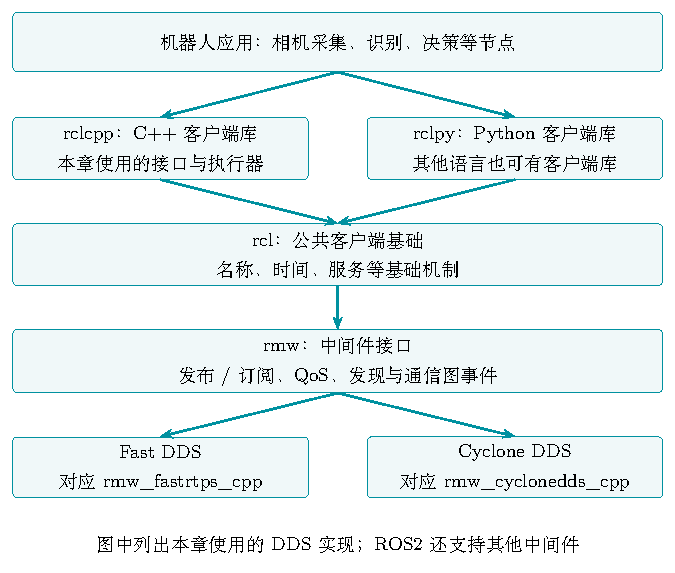
\includegraphics[width=0.8\textwidth]{ros2_arch_revised.pdf}
    \caption{本章使用的 ROS2 软件分层}
    \label{fig:ros2_arch}
\end{figure}
常见术语的含义：
\begin{itemize}
    \item \textbf{rclcpp}: ROS Client Library for C++，它是ROS2的C++客户端库，负责ROS2节点的创建、通信、生命周期管理等，我们使用的主要是这个库。
    \item \textbf{rmw}: ROS Middleware，它是ROS2的中间件接口，把上层的通信操作交给具体的中间件实现。
    \item \textbf{QoS}: Quality of Service，它是通信策略的集合，包含历史深度、可靠性、持久性等。
    \item \textbf{DDS}: Data Distribution Service，它是一种发布/订阅通信标准，Fast DDS 与 Cyclone DDS 是它的实现。ROS2 也可以通过 rmw 使用 Zenoh 等其他中间件。
\end{itemize}
\paragraph*{ROS2的节点与组件}
\textbf{ROS2的基本思想是分布式的、模块化的。}

节点（Node）是组织功能的逻辑单元。组件（Component）是可动态装载的节点实现，组件容器可在同一进程内装载多个节点。
先把下面的节点收发跑通；当图像变大、复制与调度开始影响延迟时，再按第\ref{sec:ros2-image-components}节把相邻节点组合起来。

我们可以用这个图来直观地理解ROS2的\textbf{节点}：
\begin{figure}[htbp]
    \centering
    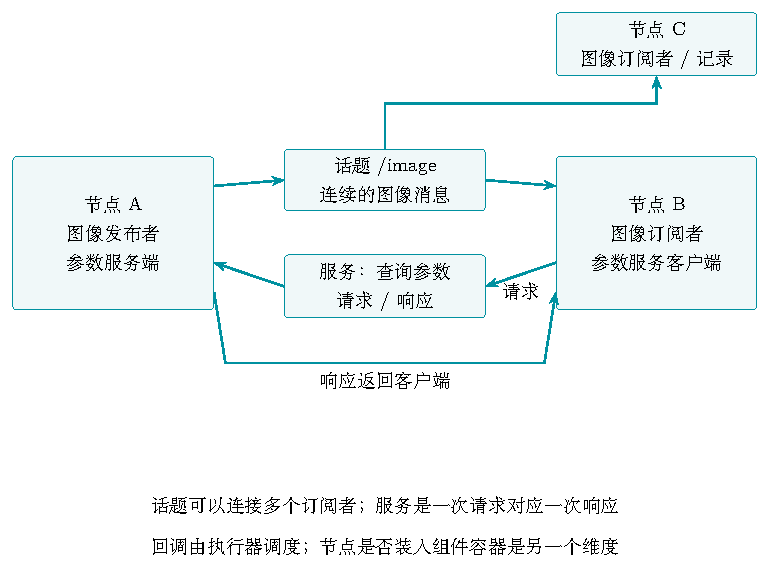
\includegraphics[width=0.8\textwidth]{ros2_node_revised.pdf}
    \caption{节点通过话题与服务通信}
    \label{fig:ros2_node}
\end{figure}

\begin{note}
如果想看节点与话题的动态关系，可以跟着官方节点教程操作：\url{https://docs.ros.org/en/humble/Tutorials/Beginner-CLI-Tools/Understanding-ROS2-Nodes/Understanding-ROS2-Nodes.html}。
\end{note}


这个图直观的反映了ROS2的模块化是依靠\textbf{节点}完成的，节点的职责可以是接收某个传感器的信息（比如相机），也可以是对数据进行处理的流程（比如对相机的图像进行滤波），也可以是提供服务（比如反馈相机的参数信息）
这些功能也可以在一个节点中完成。节点之间通过话题、服务或动作通信；回调由执行器（Executor）调度。


对于我们实际上手操作的情况下，我们更感知的操作方式有两种。
一是使用CLI tools（command-line interface），二是使用Client Libraries。
我们一般使用CLI tools来创建、运行、调试节点，而Client Libraries则用于编写节点的逻辑。

\Needspace{12\baselineskip}
\begin{example}
在终端一加载当前发行版环境后启动 talker；终端二加载相同环境，查询节点与话题：
\par\medskip\noindent\begin{minipage}{\linewidth}
\begin{tbash}
# 终端一
ros2 run demo_nodes_cpp talker
# 终端二
ros2 node list
ros2 topic info /chatter
ros2 topic echo /chatter
\end{tbash}
\end{minipage}\par\smallskip
\end{example}

\begin{exercise}
\label{ex:v2-ros-graph}
记录 /chatter 的消息类型、发布者数量。停止 talker 后重新查询，说明节点与话题的关系。
\end{exercise}

\begin{conclusion}
\begin{itemize}
\item 包组织源码和依赖，节点承担运行时功能，话题传递同类型消息。
\item 组件把节点装入进程；执行器调度回调。
\item QoS 决定通信策略，双方兼容才可能建立连接。
\end{itemize}
\end{conclusion}

\section{工作空间、节点与消息接口}
\subsubsection{创建工作空间与第一个功能包}
由图\ref{fig:ros2_arch}可以看到，rclcpp是ROS2的C++接口，我们在C++中使用这个来描述机器人的节点和节点之间的行为。
首先，你需要寻找一个你喜欢的地方新建一个文件夹，这个名字不重要，但建议起个有意义的名字。
\par\medskip\noindent\begin{minipage}{\linewidth}
\begin{tbash}
    mkdir -p ~/ros2_ws/src
    cd ~/ros2_ws/src
\end{tbash}
\end{minipage}\par\smallskip

这里把工作空间（就是文件夹）命名为ros2\_ws，并在其下创建了一个src文件夹，这个文件夹是ROS2的源代码存放的地方。

接着创建功能包（Package）。包组织代码和依赖，一个包可以包含多个节点程序。
\par\medskip\noindent\begin{minipage}{\linewidth}
\begin{tbash}
    ros2 pkg create --build-type ament_cmake my_package
\end{tbash}
\end{minipage}\par\smallskip
\Needspace{12\baselineskip}
此时的目录结构应类似：
\par\medskip\noindent\begin{minipage}{\linewidth}
\begin{tbash}
ros2_ws/
+-- src/
    +-- my_package/
        +-- CMakeLists.txt
        +-- package.xml
        +-- src/
\end{tbash}
\end{minipage}\par\smallskip

然后回到工作空间的根目录(ros2\_ws),输入以下命令编译这个包：

\par\medskip\noindent\begin{minipage}{\linewidth}
\begin{tbash}
    colcon build
\end{tbash}
\end{minipage}\par\smallskip

编译好的包会产生,build、install、log三个文件夹，其中 build 保存构建中间文件，install 保存安装后的程序、库和环境脚本，log 保存构建日志。

此时的目录结构应类似：
\par\medskip\noindent\begin{minipage}{\linewidth}
\begin{tbash}
ros2_ws/
+-- src/
|   +-- my_package/
|       +-- CMakeLists.txt
|       +-- package.xml
|       +-- src/
+-- build/
+-- install/
+-- log/
\end{tbash}
\end{minipage}\par\smallskip

稍后的完整工程给出普通 ament\_cmake 配置（代码\ref{lst:ros2-basic-cmake}），先学会显式声明依赖与安装目标。

之后我们就可以开始编写代码了。
\subsubsection{用 rclcpp 编写发布者与订阅者}

新建my\_node.cpp和my\_node.h文件。并在这两个文件中新建一个类my\_node，继承自rclcpp::Node。
Node类是ROS2提供的基础的类，我们会在这个基类上进行扩展。

其构造函数一般是用来设置节点的发布者和订阅者，绑定对应的回调函数。实现为代码\ref{lst:my_node_cpp}中的构造函数。
\paragraph*{编写发布者和订阅者}
要编写发布者和订阅者，我们需要使用rclcpp::Publisher和rclcpp::Subscription。
先在节点的类中定义一个私有成员变量，用来保存订阅者的句柄，并在构造函数中初始化。
需要注意，定义的应该是\texttt{rclcpp::Publisher<T>::SharedPtr} 与 \texttt{rclcpp::Subscription<T>::SharedPtr}即共享指针，

初始化的时候需要使用\texttt{create\_publisher<T>} 与 \texttt{create\_subscription<T>}这些模板函数。模板参数是消息类型，两者都要指定话题名和 QoS；订阅者还要提供收到消息后执行的回调。


\par\medskip\noindent\begin{minipage}{\linewidth}
\begin{tcode}
    string_publisher_ = create_publisher<std_msgs::msg::String>(
         "send",
         10
         );
\end{tcode}
\end{minipage}\par\smallskip
这个代码将类的成员变量string\_publisher\_绑定到话题名称为"send"的发布者，历史队列深度为10。这个话题名称是我随便起的，
QoS（Quality of Service，服务质量）包含历史深度、可靠性和持久性等策略。
整数 10 是 KeepLast 历史深度，不是“质量等级”。图像话题常使用 SensorDataQoS；发布与订阅策略必须兼容。
\begin{note}
把队列调大不会让处理更快。图像处理跟不上时，可能只是在积压更旧的帧。
\end{note}
这样变量string\_publisher\_所指的空间就有了一个发布者，它会发布std\_msgs::msg::String类型的消息。但是很明显你能发现它并不会发布消息，因为还没有编写发布消息的逻辑。
不妨在订阅回调中进行发布。

\par\medskip\noindent\begin{minipage}{\linewidth}
\begin{tcode}
    string_subscription_ = create_subscription<std_msgs::msg::String>(
         "receive",
         10,
         std::bind(&my_node::subscription_callback, this, std::placeholders::_1)
         );
\end{tcode}
\end{minipage}\par\smallskip
这个代码将类的成员变量string\_subscription\_绑定到话题名称为"receive"的订阅者，历史队列深度为10。
std::bind 将成员函数与当前对象 this 绑定，占位符 \texttt{std::placeholders::\_1} 接收传入的消息。
也可使用签名匹配的 lambda：\texttt{[this](std\_msgs::msg::String::SharedPtr msg)}。
这个绑定的成员函数就是所谓的订阅回调函数，它会在收到消息时被调用。然后就可以在这个函数中写收到信息之后要干什么了。
\par\medskip\noindent\begin{minipage}{\linewidth}
\begin{tcode}
void my_node::subscription_callback(const std_msgs::msg::String::SharedPtr msg)
{
 RCLCPP_INFO(get_logger(), "I hear %s", msg->data.c_str());
 auto message = std_msgs::msg::String();
 message.data = "I can hear:" + msg->data;
 string_publisher_->publish(message);
}
\end{tcode}
\end{minipage}\par\smallskip

函数体中第一行通过 RCLCPP 的日志系统打印收到的消息。这里使用 INFO 记录正常收包事件；日志级别、输出位置和高频日志限流统一见第\ref{sec:ros2-logging}节。

之后的三行是创建一个String消息类型，并设置它的data字段为收到的消息加上一段文字。然后使用刚刚定义的发布者发布这个消息。

这样我们就完成了一个最简单的ROS2节点，它可以发布和订阅消息，并且可以处理收到的消息。
接下来我们要确认消息真的经过了回调。你可以用 IDE 调试，不过先用终端跑通一遍，更容易判断是程序的问题还是 IDE 环境的问题。完整文件和运行步骤就在后面的第\ref{sec:ros2-project}节。
正式一点来说（比如在实车测试的时候），我们需要在终端中工作空间下，输入以下命令：
\par\medskip\noindent\begin{minipage}{\linewidth}
\begin{tbash}
    colcon build
    source install/setup.bash
    ros2 run my_package my_node
\end{tbash}
\end{minipage}\par\smallskip
然后打开 rqt 的 Message Publisher 与 Message Monitor，分别向话题发布与订阅消息，查看节点运行情况。完整工程跑通后，第\ref{sec:ros2-visualization}节会带我们继续用 rqt、RViz2 和 Foxglove 看曲线、图像与三维图形。

\begin{example}[能看见话题，为什么还收不到消息？]
先暂时放下自己的节点，开两个加载了相同环境的终端，用 CLI 把这个现象单独复现。终端一每秒发送一条消息，明确选择 best\_effort；终端二先要求 reliable：
\par\medskip\noindent\begin{minipage}{\linewidth}
\begin{tbash}
# 终端一
ros2 topic pub /qos_demo std_msgs/msg/String "{data: hello}" --rate 1 --wait-matching-subscriptions 0 --qos-reliability best_effort
# 终端二
ros2 topic echo /qos_demo std_msgs/msg/String --qos-reliability reliable
\end{tbash}
\end{minipage}\par\smallskip
这里把等待订阅者的数量设为 0，让发布端持续发送。你会看见 QoS 不兼容的提示，echo 收不到消息。这时别以为是ROS坏了，急着重装 ROS：只是因为发布端没有提供订阅端要求的可靠性。按 Ctrl+C 停止 echo，再把它的要求改为 best\_effort：
\par\medskip\noindent\begin{minipage}{\linewidth}
\begin{tbash}
ros2 topic echo /qos_demo std_msgs/msg/String --qos-reliability best_effort --once
ros2 topic info /qos_demo --verbose
\end{tbash}
\end{minipage}\par\smallskip
这次应收到 hello；详细信息还能看到各个端点的策略。可靠性只是其中一项，其他策略也必须兼容。结束后停止发布进程，避免它影响后面的实验。
\end{example}
\begin{exercise}
\label{ex:v2-ros-qos}
把发布者改为 reliable、订阅者保留 best\_effort，预测能否收包并实际验证；说明为什么双方策略不必完全相同。
\end{exercise}
\begin{note}
QoS 策略与兼容性表见官方文档：\url{https://docs.ros.org/en/humble/Concepts/Intermediate/About-Quality-of-Service-Settings.html}。
\end{note}

\subsubsection{用定时器周期发布消息}
\begin{note}
日志中的时间用于排查事件顺序。Unix 时间以 UTC 1970 年 1 月 1 日为纪元；ROS 时间还可能由仿真时钟提供，跨节点比较前先确认时钟来源。
\end{note}
这个非常简单，定义rclcpp::TimerBase 类型，然后用C++中的 \texttt{chrono} 库来提供定时器时间，再使用\texttt{create\_wall\_timer}绑定一个函数作为回调函数即可。
\par\medskip\noindent\begin{minipage}{\linewidth}
\begin{tcode}
    //定义成员变量
    rclcpp::TimerBase::SharedPtr timer_;
    //构造函数
    timer_ = create_wall_timer(
        std::chrono::milliseconds(1000), // 定时器间隔
        std::bind(&my_node::timer_callback, this)); // 回调函数
    //回调函数
    void my_node::timer_callback()
    {
        RCLCPP_INFO(get_logger(), "timer count=%d", ++cnt_);
        auto time_msg = std_msgs::msg::String();
        time_msg.data = "Now is " + std::to_string(cnt_);
        timer_publisher_->publish(time_msg);
    }
\end{tcode}
\end{minipage}\par\smallskip
这个回调函数会每秒钟被调用一次，打印一下回调计数，并发布计数消息。

\subsubsection{定义、生成与使用自定义消息}
自定义消息由字段组成。字段可使用基本类型，也可使用 ROS2 已有的消息类型，例如 \path{std_msgs/Header}。
以实际应用例子，我们的机器人在自瞄时传输瞄准的装甲板数据时，需要知道id(敌方装甲板的编号)，yaw(装甲板的偏航角度)等信息。
同时我们还要知道识别到的时间信息。与其把它们塞进一个难以检查的字符串，不如定义一条带类型的消息，让收发两边对字段和单位有共同约定。


在ROS 2中，使用RCLCPP接口创建自定义消息类型需要以下步骤：

1. 创建自定义消息包

首先，创建一个专门用于存放自定义消息的包。例如，创建一个名为my\_msgs的包：
\par\medskip\noindent\begin{minipage}{\linewidth}
\begin{tbash}
    ros2 pkg create --build-type ament_cmake my_msgs
\end{tbash}
\end{minipage}\par\smallskip

然后在该包中创建msg目录，用于存放自定义消息文件。


\begin{note}
包名如 \texttt{my\_msgs} 使用小写字母、数字和下划线，并以字母开头。消息文件名如 \texttt{My.msg} 以大写字母开头，只含字母和数字。两种名字不要混淆。
\end{note}


2. 定义自定义消息

在 msg 目录中创建 My.msg 文件，定义消息结构；yaw 在本例中以弧度表示。
\par\medskip\noindent\begin{minipage}{\linewidth}
\begin{tbash}
    std_msgs/Header header
    uint8 id
    float64 yaw
    bool detect_success
\end{tbash}
\end{minipage}\par\smallskip

3. 修改CMakeLists.txt文件和package.xml文件

建议直接看完整工程的代码\ref{lst:xml_2}

4. 编译自定义消息

在工作空间中运行以下命令以编译自定义消息：
\par\medskip\noindent\begin{minipage}{\linewidth}
\begin{tbash}
    colcon build --packages-select my_msgs
    source install/setup.bash
\end{tbash}
\end{minipage}\par\smallskip

编译后以 \texttt{\#include <my\_msgs/msg/my.hpp>} 引用生成的头文件。

5. 在节点中使用自定义消息

在其他节点中使用自定义消息时，需要在CMakeLists.txt中添加对my\_msgs的依赖，并在代码中包含自定义消息的头文件。就像其他ROS2自带的消息类型一样。


\begin{example}
完成完整工程的消息包后，加载工作空间环境，检查定义是否生成：
\par\medskip\noindent\begin{minipage}{\linewidth}
\begin{tbash}
source ~/ros2_ws/install/setup.bash
ros2 interface show my_msgs/msg/My
\end{tbash}
\end{minipage}\par\smallskip
输出应包含 header、id、yaw、detect\_success 四个字段；Header 的内部字段会展开显示。
\end{example}

\begin{exercise}
\label{ex:v2-ros-message}
给消息加入 float64 distance 字段，重新构建消息包，检查接口输出。约定 distance 单位为米。
\end{exercise}
\subsubsection{常用消息类型与接口查询}

1.\ std\_msgs

常用消息包括 \texttt{String}、\texttt{Int32}、\texttt{Float64} 等标量与数组类型。
\texttt{std\_msgs/Header} 含 \texttt{stamp}（时间戳）与 \texttt{frame\_id}（坐标系标识），几何与传感器消息常内嵌该头。

除了 std\_msgs，常用消息集合 common\_msgs 中还有 \texttt{geometry\_msgs}、\texttt{nav\_msgs}、\texttt{sensor\_msgs} 等。

2.geometry\_msgs。最常用的几何消息类型，定义了描述机器人状态的各种类型，比如点、速度、加速度、位姿等。

Vector3 用三个 float64 描述三维向量，例如速度或方向；表示空间中的位置点通常用 Point。两者看起来都有 x、y、z，不过表示的实际物理含义不同。带 Stamped 后缀的类型还提供 Header，让我们知道数据来自哪个坐标系、对应哪个时刻。
Quaternion、QuaternionStamped是传输四元数的消息类型。
Transform、TransformStamped是传输坐标系变换关系的消息类型。

3.sensor\_msgs。包含了传感器数据，包括图像、激光、雷达、IMU等。

主要用的就上面三种消息类型。



更多更详细内容请参考官方文档。

\begin{example}
完成本章完整工程后，查看接口定义并只接收一次定时器消息：
\par\medskip\noindent\begin{minipage}{\linewidth}
\begin{tbash}
source /opt/ros/humble/setup.bash
source ~/ros2_ws/install/setup.bash
ros2 interface show my_msgs/msg/My
ros2 interface show geometry_msgs/msg/Vector3
ros2 interface show geometry_msgs/msg/Point
ros2 interface show sensor_msgs/msg/Image
ros2 topic echo /timer_ --once
\end{tbash}
\end{minipage}\par\smallskip
先对照 Vector3 与 Point 的注释，再看看 Image 除了像素数据还有哪些描述字段。Header 的 frame\_id 只是坐标系标识，写一个名字不会替你完成坐标变换：后面使用 tf2 时才会把坐标系之间的关系连起来。
\begin{note}
Image 包含 height、width、encoding、step 和 data 等字段，CompressedImage 则描述压缩格式和压缩后的数据，别把它们混在一起。需要核对原始定义时，可以直接查看包中的消息文件：
\par\medskip\noindent\begin{minipage}{\linewidth}
\begin{tbash}
cat "$(ros2 pkg prefix --share sensor_msgs)/msg/Image.msg"
\end{tbash}
\end{minipage}\par\smallskip
这里查看的是 \texttt{sensor\_msgs::msg::Image} 的消息定义；它与\texttt{CompressedImage}是两个不同的类型。
\end{note}
\end{example}

\begin{exercise}
\label{ex:v2-ros-timer}
将定时器间隔改为 500 ms，重编译并用 ros2 topic hz /timer\_ 检查频率；再解释消息中的时间戳与计数器有何不同。
\end{exercise}

\begin{conclusion}
\begin{itemize}
\item 编辑 src 中的文件，回到工作空间根目录编译。
\item build 是构建过程，install 是运行入口，使用前加载 setup.bash。
\item 自定义接口先声明字段与依赖，再生成代码；订阅、发布和定时器句柄要持续存活。
\end{itemize}
\end{conclusion}

\subsubsection{服务调用与后续工具}
这部分是一些ROS2的较高级内容，主要是介绍名字和基本用途。
可以在需要的时候查找对应关键词。

\textbf{功能:}
\begin{enumerate}
    \item ROS2 launch，可以用来启动多个节点，并设置参数。用于启动复杂的系统。
    \item service的代码实现
    \item ROS2参数，可以通过launch文件设置参数，也可以在代码中设置参数。
    \item rosbag 用于记录和重放ROS2的消息。这点对于调试和分析非常有用，可以做到在家就能调试。
    \item 通过ROS2组件的形式启动ROS2节点。
\end{enumerate}

\textbf{包:}
\begin{enumerate}
    \item cv\_bridge 包，用于ROS2和OpenCV之间的互相转换。
    \item camera\_calibration 用于相机标定，配合参数管理与 image\_proc 图像校正；完整流程见第\ref{sec:ros2-camera-calibration}节。
    \item tf2 包，提供了一个坐标变换的框架。
    \item RViz2 用于可视化坐标系、位姿、轨迹和图形消息；rqt 与 Foxglove 的曲线、图像、标注和回放也会在第\ref{sec:ros2-visualization}节练习。
    \item moveit2 包，用于机械臂控制。
    \item navigation2 包，用于导航。
\end{enumerate}

\begin{example}
使用已安装的 demo 服务。终端一运行服务端，终端二调用后应得到 sum: 5。
\par\medskip\noindent\begin{minipage}{\linewidth}
\begin{tbash}
# 两个终端都先加载同一发行版环境
# 终端一
ros2 run demo_nodes_cpp add_two_ints_server
# 终端二
ros2 service call /add_two_ints example_interfaces/srv/AddTwoInts "{a: 2, b: 3}"
\end{tbash}
\end{minipage}\par\smallskip
\end{example}

\begin{exercise}
\label{ex:v2-ros-service}
用服务列表和接口查询命令查出该服务的请求、响应字段；说明这种一次请求与持续发布话题的区别。
\end{exercise}

